Nesse capítulo, apresentamos os fundamentos da Análise de Redes Sociais. A análise de redes sociais (ARS) é uma abordagem que tem suas raízes na Sociometria e na Teoria dos Grafos, que são de viés matemático, para analisar relações sociais \cite{2015_Recuero_BOOK}. A ideia central é que os indivíduos, ou atores sociais, estão inseridos em estruturas complexas de relações com outros atores, e essas estruturas têm um papel fundamental no comportamento e na visão de mundo desses indivíduos.

\section{Teoria dos Grafos}
A Teoria dos Grafos é um framework matemático que estuda as relações entre objetos e as conexões entre eles. As origens desta teoria estão no trabalho de Euler e na solução que ele propôs para o enigma das Pontes de Königsberg. A história relata que a cidade de Königsberg seria atravessada por sete pontes e que popularmente havia um desafio de desenhar um caminho por ela onde cada uma das pontes seria atravessada uma única vez. Euler teria demonstrado que tal desafio era impossível de ser resolvido utilizando um grafo, dando assim origem à teoria.

Em \citeonline{2017_Recuero}, a autora discute a importância da ARS e da Teoria dos Grafos para a compreensão das redes sociais online. Ela explica que a ARS permite a análise sistemática de grupos sociais a partir de sua estrutura, através de medidas específicas. A autora também destaca que a análise de redes sociais nasce de um ramo interdisciplinar de pesquisa, cujas bases podem ser encontradas nas mais variadas ciências, principalmente no início do século XX, particularmente, a partir da década de 1930.

Um conceito fundamental na Teoria dos Grafos é o de um "grafo", que é uma estrutura composta por "vértices" (ou "nós") e "arestas" que conectam esses vértices. Formalmente, um grafo $G$ é definido como um par ordenado $G := (V, E)$ compreendendo um conjunto $V$ de vértices ou nós juntamente com um conjunto $E$ de arestas ou arcos, que são pares de vértices \cite{1976_Bondy_BOOK}.

Os grafos podem ser categorizados como direcionados ou não direcionados. Em um grafo direcionado, as arestas têm uma direção associada, indicando uma relação unidirecional. Em contraste, em um grafo não direcionado, as arestas não têm direção, sugerindo uma relação bidirecional \cite{2000_West_BOOK}. Em termos de redes sociais, um exemplo de grafo direcionado seria o Twitter (onde um usuário pode seguir outro sem ser seguido de volta), enquanto um exemplo de grafo não direcionado seria o Facebook (onde a amizade é sempre mútua).

\begin{figure}
	\centering
	\begin{tikzpicture}[node distance=2cm]

		% Estilos para os nós e arestas
		\tikzstyle{user} = [circle, draw=black, fill=blue!30, minimum size=1cm, inner sep=0pt]
		\tikzstyle{follow} = [thick,->,>=stealth]

		% Usuários
		\node (A) [user, label=below:Ana] {};
		\node (B) [user, right=of A, label=below:Bob] {};
		\node (C) [user, above right=of A, label=right:Carlos] {};
		\node (D) [user, below right=of A, label=right:Diana] {};
		\node (E) [user, below=of D, label=below:Eva] {};
		\node (F) [user, left=of E, label=below:Felipe] {};
		\node (G) [user, above left=of F, label=left:Gabriel] {};

		% Relações de "seguir"
		\draw[follow] (A) -- (B);
		\draw[follow] (B) -- (C);
		\draw[follow] (C) -- (D);
		\draw[follow] (D) -- (A);
		\draw[follow] (A) -- (C);
		\draw[follow] (B) -- (D);
		\draw[follow] (E) -- (D);
		\draw[follow] (E) -- (F);
		\draw[follow] (F) -- (G);
		\draw[follow] (G) -- (A);

	\end{tikzpicture}
	\caption{Ilustração de uma rede social com usuários seguindo uns aos outros. O subgrafo formado por Ana, Bob, Carlos e Diana representa um clique, pois todos estão conectados entre si. O caminho de Eva para Ana passa por Diana e Gabriel.}
\end{figure}

Outro conceito importante é o "grau" de um vértice, que é o número de arestas conectadas a ele. Em um grafo direcionado, distinguimos entre o "grau de entrada" (o número de arestas que entram no vértice) e o "grau de saída" (o número de arestas que saem do vértice). O grau de um vértice pode ser usado para medir sua importância ou influência dentro da rede \cite{2010_Newman_BOOK}.

Um "caminho" em um grafo é uma sequência de vértices na qual cada vértice é conectado ao próximo por uma aresta. O "comprimento" de um caminho é o número de arestas que ele contém. Este conceito é crucial para entender como a informação ou influência pode se propagar através da rede \cite{2010_Easley_BOOK}.

A "conectividade" de um grafo é uma medida de quão integrada ou unida é a rede. Um grafo é dito "conectado" se houver um caminho entre cada par de vértices \cite{2000_West_BOOK}.

Um "subgrafo" é um grafo formado a partir de um conjunto de vértices e arestas de um grafo maior. Os subgrafos podem ser usados para estudar partes específicas de uma rede \cite{2000_West_BOOK}.

Recuero também enfatiza a diferença entre redes sociais e sites de rede social. Enquanto uma rede social está relacionada à percepção de um grupo social determinado pela sua estrutura (a “rede”), que é geralmente oculta, pois só está manifesta nas interações, as ferramentas sociais na internet são capazes de publicizar e influenciar essas estruturas sociais. Assim, o Facebook, por si só, não apresenta redes sociais. É o modo de apropriação que as pessoas fazem dele que é capaz de desvelar redes que existem ou que estão baseadas em estruturas sociais construídas por essas pessoas.

Portanto, a Teoria dos Grafos e a Análise de Redes Sociais são ferramentas essenciais para a compreensão das complexas redes de interações sociais que se formam tanto no mundo offline quanto online. Elas permitem uma visão mais profunda e sistemática das relações sociais, contribuindo para uma melhor compreensão dos fenômenos sociais.

\subsection*{Grafos Sociais}

Um dos primeiros desenvolvimentos na análise de redes foi o trabalho do sociólogo Georg Simmel no início do século XX. Simmel aplicou os princípios da teoria dos grafos às relações sociais, argumentando que as estruturas sociais surgem a partir dos padrões de interação entre os indivíduos \cite[]{2021_Hollstein}. Desde então, a análise de redes tem sido aplicada em uma ampla gama de campos, incluindo ciência da computação, física, biologia e ciências sociais, entre outros.

Simmel foi pioneiro em determinar a interação social como o bloco de construção básico da sociologia, indo além de seus contemporâneos, como Spencer. Ele argumentou que para entender o comportamento social, devemos estudar os padrões de interação, oferecendo insights penetrantes sobre a dinâmica das relações sociais. Embora Simmel nunca tenha usado o termo "rede social", muitos analistas de rede o consideram um precursor importante da abordagem de rede social.

Além disso, a análise de redes tem sido usada para entender a estrutura e a dinâmica de "redes escuras", como redes de criminosos ou terroristas. A análise de redes também tem sido aplicada para entender a estrutura e a dinâmica das organizações e como a estrutura da rede pode afetar a eficácia e a eficiência organizacional.

No entanto, apesar do rápido crescimento da análise de redes nas últimas duas décadas, as críticas à abordagem também aumentaram. Alguns críticos argumentam que a análise de redes pode ser excessivamente determinística, ignorando a agência individual e a complexidade das relações sociais \cite{1991_Scott}. Além disso, a análise de redes pode ser desafiadora devido à dificuldade de coletar dados completos e precisos sobre redes sociais.

A análise de redes sociais tem sido criticada por sua falta de consideração pelos aspectos qualitativos das redes sociais e por sua tendência a simplificar as complexidades das interações sociais \cite{2013_Gruzd}. Além disso, a análise de redes sociais é frequentemente criticada por sua falta de consideração pelos aspectos contextuais das redes sociais e por sua ênfase excessiva em padrões estruturais.

Essas críticas destacam a necessidade de abordagens mais holísticas e integradas para a análise de redes sociais, que levem em consideração tanto os aspectos quantitativos quanto qualitativos das redes sociais, bem como os contextos sociais e culturais em que essas redes estão inseridas.

\subsection*{Modularidade}

A modularidade é uma métrica que quantifica a estrutura de comunidades em redes. Introduzida por \cite{2004_Newman}, a modularidade mede a diferença entre a fração de arestas que caem dentro de comunidades e a fração esperada se as arestas fossem distribuídas ao acaso, mantendo a distribuição de grau dos nós. Valores de modularidade próximos a 0 indicam que a divisão da rede em comunidades não é melhor do que uma atribuição aleatória, enquanto valores próximos a 1 indicam uma divisão forte em comunidades. Em termos práticos, uma rede com alta modularidade tem mais conexões dentro de suas comunidades e menos conexões entre comunidades diferentes do que seria esperado por acaso.

Para ilustrar, imagine uma rede social de estudantes de uma universidade, onde os estudantes pertencem a diferentes departamentos, como Engenharia, Artes e Ciências. Se os estudantes de Engenharia tendem a interagir mais frequentemente entre si, e o mesmo acontece com os estudantes de Artes e Ciências, então essa rede teria uma alta modularidade. Isso porque há uma densidade maior de conexões dentro de cada departamento (comunidade) do que entre departamentos diferentes. Em contraste, se os estudantes interagissem aleatoriamente, independentemente de seus departamentos, a modularidade seria próxima de 0, indicando uma ausência de estrutura comunitária clara.

\begin{figure}
	\centering
	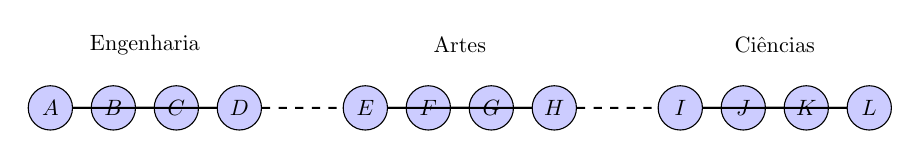
\begin{tikzpicture}[scale=0.8, every node/.style={scale=0.8}]
		% Styles
		\tikzstyle{vertex}=[circle,draw=black,fill=blue!20,minimum size=20pt,inner sep=0pt]
		\tikzstyle{edge}=[draw,thick,-]

		% Nodes for Engenharia
		\foreach \name/\x in {A/1,B/2,C/3,D/4}
		\node[vertex] (\name) at (\x,4) {$\name$};

		% Nodes for Artes
		\foreach \name/\x in {E/6,F/7,G/8,H/9}
		\node[vertex] (\name) at (\x,4) {$\name$};

		% Nodes for Ciências
		\foreach \name/\x in {I/11,J/12,K/13,L/14}
		\node[vertex] (\name) at (\x,4) {$\name$};

		% Connect nodes in Engenharia
		\foreach \source/\dest in {A/B, B/C, C/D, D/A, A/C, B/D}
		\path[edge] (\source) -- (\dest);

		% Connect nodes in Artes
		\foreach \source/\dest in {E/F, F/G, G/H, H/E, E/G, F/H}
		\path[edge] (\source) -- (\dest);

		% Connect nodes in Ciências
		\foreach \source/\dest in {I/J, J/K, K/L, L/I, I/K, J/L}
		\path[edge] (\source) -- (\dest);

		% Connect nodes between departments
		\path[edge, dashed] (D) -- (E);
		\path[edge, dashed] (H) -- (I);

		% Labels
		\node[align=center] at (2.5,5) {Engenharia};
		\node[align=center] at (7.5,5) {Artes};
		\node[align=center] at (12.5,5) {Ciências};
	\end{tikzpicture}
	\caption{Ilustração da modularidade em uma rede de estudantes de diferentes departamentos. Os nós representam estudantes, as arestas sólidas representam interações dentro dos departamentos e as arestas tracejadas representam interações entre departamentos.}
\end{figure}

\subsection*{Centralidade e Comunidades}

Um método comum usado na análise de redes é a análise de centralidade, que mede a importância dos nós na rede com base em sua posição e conexões dentro da rede \cite[]{1978_Freeman}. Medidas de centralidade podem ajudar a identificar atores-chave na rede, ou nós que desempenham papéis importantes como porteiros, conectores ou intermediários entre diferentes partes da rede.

Outro método importante na análise de redes é a detecção de comunidades, que identifica grupos de nós que estão mais densamente conectados entre si do que com o restante da rede \cite[]{2004_Newman}. A detecção de comunidades pode ajudar a identificar grupos de indivíduos com atributos ou comportamentos semelhantes, ou grupos que são mais suscetíveis à propagação de informações ou influências.

\subsection*{Algoritmo de Louvain}

A partir dos conceitos de centralidade, comunidade e modularidade, é possivel criar heurísticas mais especializadas para interpretar os grafos das redes, por exemplo, o algoritmo de Louvain é uma metodologia heurística para detecção de comunidades em grandes redes. Desenvolvido por \citeonline{2008_Blondel}, o algoritmo tem como principal objetivo identificar grupos de nós em redes que estão mais densamente conectados entre si do que com o restante da rede. A ideia central é maximizar a modularidade da forma mais eficiente possível.

O algoritmo opera em duas fases que são repetidas iterativamente. Na primeira fase, cada nó é atribuído à sua própria comunidade. Em seguida, para cada nó, o algoritmo avalia a ganho de modularidade ao mudar a comunidade desse nó para a comunidade de seus vizinhos. Se um aumento na modularidade é observado, o nó é colocado na comunidade que proporciona esse aumento. Este processo é repetido para todos os nós até que nenhum aumento na modularidade possa ser alcançado. Na segunda fase, as comunidades encontradas na primeira fase são agregadas para formar uma nova rede de comunidades, onde os nós da nova rede representam as comunidades e os links representam as conexões entre comunidades da rede original. Estas duas fases são repetidas até que a modularidade se estabilize.

No contexto de estudos sobre câmaras de eco, o algoritmo de Louvain é particularmente relevante. Câmaras de eco são, por definição, grupos de indivíduos que compartilham e reforçam opiniões semelhantes, minimizando a exposição a opiniões divergentes. A capacidade do algoritmo de Louvain de identificar comunidades densamente conectadas em redes torna-o uma ferramenta valiosa para detectar esses grupos. Ao identificar comunidades que interagem predominantemente entre si, os pesquisadores podem isolar e estudar essas câmaras de eco, compreendendo melhor sua formação, evolução e impacto na disseminação de informações.

\section{Aplicações da Análise de Redes}

A análise de redes tem sido aplicada em uma ampla gama de campos, além das redes sociais, com aplicações que vão desde redes de transporte até a neurociência. Nesta seção, vamos destacar algumas contribuições notáveis.

No campo do transporte, a análise de redes tem sido usada para estudar o fluxo de tráfego nas estradas e identificar áreas de gargalo que podem ser melhoradas para aumentar a eficiência do tráfego \cite[]{2012_Levinson}. Por exemplo, \citeonline{2010_Bierlaire} aplicaram a análise de redes para otimizar o sistema de transporte público, reduzindo o tempo de viagem e melhorando a eficiência do serviço. No campo acadêmico, a análise de redes tem sido aplicada para estudar as redes de coautoria na publicação acadêmica. \citeonline{2001_Newman} utilizou a análise de redes para estudar os padrões de colaboração entre autores e a emergência de comunidades de pesquisa. No campo organizacional, a análise de redes tem sido usada para compreender a estrutura de padrões de comunicação formais e informais em organizações. \citeonline{2004_Cross_BOOK} utilizaram a análise de redes para entender como os indivíduos influenciam os processos de tomada de decisão e a emergência de estruturas de poder dentro das organizações. Na biologia, a análise de redes tem sido usada para estudar redes de interação de proteínas, redes regulatórias de genes e redes metabólicas \citeonline{2004_Barabasi} utilizaram a análise de redes para entender como as proteínas interagem entre si em uma célula, fornecendo insights sobre como as doenças afetam essas interações.
\begin{figure}[!htb]
	\caption{Imagem ilustrativa de uma rede de interação de proteínas}
	\label{fig:network_proteins}
	\centering
	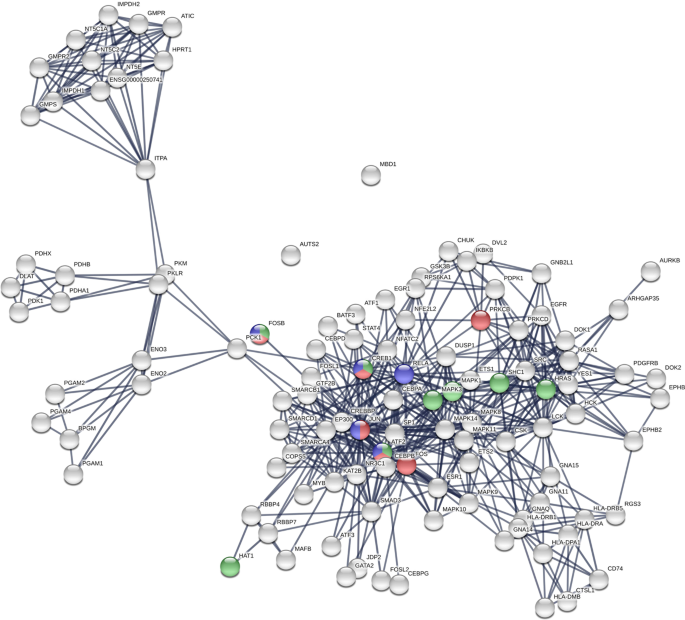
\includegraphics[scale=0.5]{network_proteins.png}
	\fdireta{2004_Barabasi}
\end{figure}
A análise de redes também tem sido usada em neurociência para estudar redes cerebrais. Por exemplo, pesquisadores têm utilizado a análise de redes para entender como diferentes regiões do cérebro interagem entre si, o que pode ajudar a entender doenças como a esquizofrenia e o Alzheimer \cite[]{2009_Bullmore}.
\begin{figure}[!htb]
	\caption{Imagem ilustrativa de uma rede de interação de proteínas}
	\label{fig:network_brain}
	\centering
	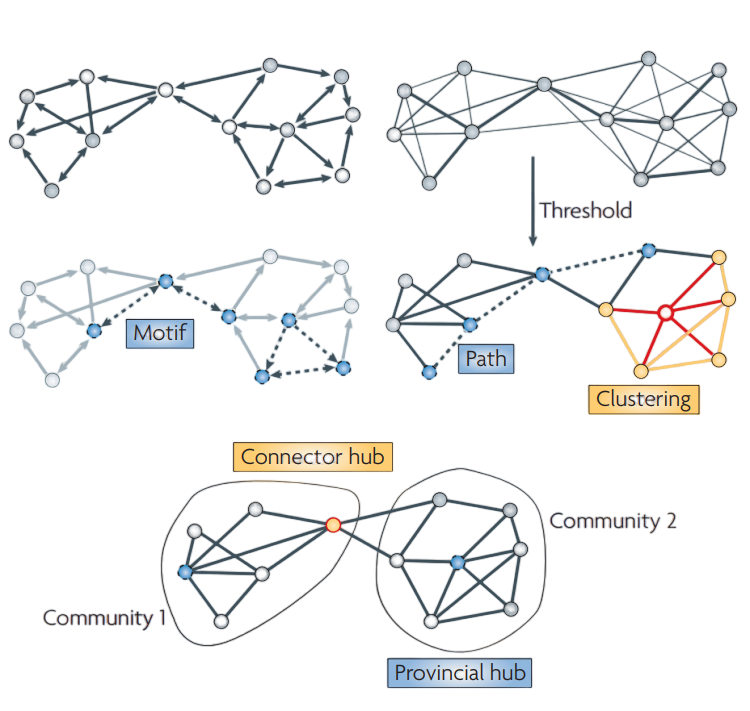
\includegraphics[scale=0.25]{network_brain.png}
	\fdireta{2009_Bullmore}
\end{figure}

\subsection*{Análise de Redes Sociais Online}

Outra importante aplicação da análise de redes está no estudo de comunidades online e mídias sociais. O crescimento exponencial de plataformas online e redes sociais tem fornecido aos pesquisadores vastas quantidades de dados para analisar a dinâmica dessas comunidades. Por exemplo, um estudo de utilizou a análise de redes para investigar a estrutura e dinâmica das comunidades de discussão online no Reddit. O estudo constatou que as comunidades exibiam uma estrutura hierárquica com subcomunidades distintas que se formavam em torno de tópicos específicos. Outro estudo de \citeonline{2011_Quercia_IP} utilizou a análise de redes para estudar a influência de relacionamentos sociais na propagação de informações no Twitter. O estudo constatou que a estrutura da rede social influenciava a propagação de informações, sendo que clusters densamente conectados tinham maior probabilidade de promover a difusão de informações do que clusters esparsamente conectados.

Em conclusão, a análise de redes é uma ferramenta poderosa para analisar sistemas complexos e compreender as relações entre seus componentes. Ela tem suas origens na teoria dos grafos e se desenvolveu em um campo multidisciplinar com aplicações em várias áreas, como redes sociais, comunidades online, epidemiologia, ecologia e transporte. A aplicação da análise de redes em redes sociais tem levado a insights importantes sobre a estrutura e dinâmica dessas redes e tem ajudado os pesquisadores a compreender os mecanismos de influência social e a propagação de informações. O uso da análise de redes em outros campos também tem levado a descobertas importantes e tem o potencial de aprimorar nossa compreensão dos sistemas que moldam nosso mundo.

\subsection*{Análise de Redes Sociais no Brasil}

A Análise de Redes Sociais (ARS) emergiu como uma ferramenta poderosa e cada vez mais popular para analisar a estrutura e a dinâmica das redes sociais. Utilizada para estudar uma variedade de fenômenos, como comportamento organizacional, redes políticas, crime e inovação, a ARS tem demonstrado ser uma metodologia extremamente versátil. No Brasil, a relevância da ARS é evidenciada em múltiplos contextos e áreas de estudo, incluindo o planejamento urbano, a avaliação de políticas públicas, a compreensão das dinâmicas de migração e a análise de preconceitos e divisões sociais nas redes sociais.

Um dos aspectos que torna a ARS especialmente relevante no Brasil é o alto uso de redes sociais pela população. O Brasil é um dos países com maior número de usuários de redes sociais no mundo, criando um vasto campo de dados que pode ser analisado através da ARS. Além disso, a diversidade cultural e regional do Brasil, com suas muitas diferenças locais, proporciona um cenário complexo que a ARS pode ajudar a decifrar. Ao identificar padrões de interação e circulação de informações nas redes sociais, a ARS pode revelar como essas diferenças regionais e culturais se manifestam online.

Além disso, o Brasil enfrenta uma série de questões sociais complexas e uma alta polarização política, aspectos que são frequentemente expressos e amplificados nas redes sociais. A ARS pode ser uma ferramenta valiosa para entender a formação e a dinâmica dessas polarizações, assim como para estudar a formação de grupos de opinião e a disseminação de informações (ou desinformação). Por último, eventos de grande escala, como a Copa do Mundo, as Olimpíadas ou as eleições presidenciais, geram uma enorme quantidade de atividade nas redes sociais, proporcionando oportunidades únicas para a aplicação da ARS.

Diante deste cenário, este capítulo apresenta um resumo breve da de algumas contribuições relevantes que utilizam a ARS no Brasil, começando com uma revisão de suas principais contribuições teóricas e metodológicas. Em seguida, ele discute os desafios atuais e futuros na aplicação desta abordagem no contexto brasileiro, com o objetivo de explorar como a ARS pode continuar a fornecer insights valiosos em meio à constante evolução das redes sociais.

Do ponto de vista teórico, a Análise de Redes Sociais (ARS) tem sido fundamental para entender como as redes sociais influenciam a formação de opiniões, a disseminação de informações e a mobilização social. Um exemplo relevante é o estudo de \citeonline{2021_Recuero}, que investigaram a polarização em torno do uso da cloroquina para tratar a COVID-19 no Brasil, analisando dados do Twitter. O estudo mostrou como a ARS pode ser aplicada para identificar câmaras de eco e a formação de bolhas de filtro, onde usuários com diferentes posições políticas e ideológicas têm acesso a fontes de informação divergentes. A análise revelou que a narrativa sobre a cloroquina foi capturada pela disputa política, com diferentes grupos compartilhando e reforçando suas crenças por meio das redes sociais. O trabalho de Recuero também informa a metodologia de \citeonline{2021_Kalinke} que explora a topologia da rede entre usuários do Twitter apoiadores e críticos ao governo de Jair Bolsonaro em relaçao as 100 mil mortes por COVID-19. O estudo utilizou métricas de centralidade para identificar clusters de usuários que não interagem entre membros fora das suas bolhas, o que contribui com um discurso reverberado por câmaras de eco.

Além disso, a ARS tem sido usada para investigar como as redes sociais podem facilitar a disseminação de informações falsas ou enganosas, o que tem implicações significativas para a democracia e a saúde pública. Um estudo interessante foi conduzido por \citeonline{2020_Lima}, que analisaram a circulação de informações sobre a COVID-19 no Twitter. Eles utilizaram a ARS para identificar padrões de compartilhamento de conteúdo e relacionamentos entre usuários. O estudo revelou que a desinformação estava fortemente associada ao consumo de veículos hiperpartidários e ao conteúdo de mídia social, enquanto a informação factual estava mais associada a veículos jornalísticos e institucionais. Isso demonstra como a ARS pode contribuir para a compreensão dos mecanismos de propagação da desinformação nas redes sociais e auxiliar na identificação de estratégias para mitigar esse problema.

Outro estudo relevante é o de \citeonline{2015_Coelho}, que analisou a rede de interações no Twitter durante o \#ProtestodosPintas em Natal (RN). O estudo encontrou que os significados construídos nas redes sociais sobre o protesto foram em grande parte negativos, com a rede sendo articulada em torno de 2 perfis. Este estudo demonstra como a ARS pode ser usada para analisar a opinião pública e a formação de consenso (ou dissensão) em torno de eventos específicos.

Esses exemplos ilustram como a ARS tem contribuído para avanços teóricos e metodológicos na compreensão das redes sociais no contexto brasileiro. As aplicações da ARS mencionadas nos estudos citados fornecem insights valiosos sobre a formação de opiniões, a disseminação de informações, a polarização política e a estrutura das redes sociais em diferentes contextos. Ao utilizar técnicas da ARS e analisar os dados específicos desses estudos, os pesquisadores foram capazes de desvendar padrões, identificar comunidades e compreender as interações sociais e políticas nas redes sociais.

Finalmente, a diversidade cultural e regional do Brasil apresenta um desafio adicional. Como mencionado anteriormente, o Brasil é um país de grande diversidade, com muitas diferenças locais. Isso significa que a análise de redes sociais no Brasil deve levar em consideração essa diversidade, adaptando-se às especificidades de diferentes contextos regionais e culturais.

Com base nos dados extremamente localizados do Colab, nos quais os usuários interagem e criam eventos relacionados a problemas específicos em suas cidades, como buracos nas vias, calçadas irregulares, descarte irregular de lixo, vazamentos de água e iluminação pública, é possível obter insights valiosos tanto no âmbito social quanto político.

Em termos sociais, a análise das interações e dos padrões de engajamento dos usuários pode revelar informações sobre a coesão social e a formação de grupos de interesse em nível local. Por exemplo, ao examinar as postagens sobre problemas específicos, como buracos nas vias, é possível identificar redes de interação entre os usuários que compartilham preocupações semelhantes. Essas redes podem revelar comunidades de interesse e fornecer insights sobre a participação cívica local e a busca de soluções colaborativas para questões cotidianas.

Do ponto de vista político, a análise das interações políticas no Colab pode fornecer informações sobre a polarização e a formação de grupos de opinião em nível local. Por exemplo, ao examinar as postagens relacionadas a políticas públicas, é possível identificar padrões de interação entre usuários com diferentes posições políticas. Esses padrões podem ajudar a compreender a dinâmica da polarização política em nível local e como isso influencia a deliberação pública e a tomada de decisões políticas.

A análise dos dados do Colab sob uma perspectiva da ARS permite adquirir insights valiosos em diversos aspectos sociais e políticos, desde a coesão social em nível local até a dinâmica da polarização política. Ao estabelecer essas conexões, é possível obter uma compreensão mais abrangente e contextualizada das redes sociais e de como elas impactam a vida cotidiana e a tomada de decisões nas comunidades.

\section{Compreendendo Câmaras de Eco e suas implicações}
\label{05_echochambers}
As mídias sociais revolucionaram a forma como as pessoas se comunicam e interagem umas com as outras. No entanto, o lado negativo dessa revolução é a crescente polarização e isolamento das pessoas em câmaras de eco. Uma câmara de eco pode ser definida como um sistema fechado em que as pessoas interagem apenas com aquelas que compartilham das mesmas crenças, valores e ideologias, enquanto ignoram ou suprimem ativamente pontos de vista opostos \cite[]{2015_Bakshy}. O termo "câmara de eco" tem origem no conceito de uma câmara de reverberação sonora, onde as ondas sonoras são refletidas entre as paredes, amplificando e distorcendo o som original.

Câmaras de eco podem ter sérias implicações para a sociedade, pois limitam a exposição a perspectivas diversas, levando ao reforço de crenças existentes e à exclusão de pontos de vista alternativos \cite[]{2001_Sunstein_BOOK}. Isso pode contribuir para a criação de uma divisão ideológica, que pode prejudicar o diálogo construtivo e o compromisso, resultando em uma sociedade polarizada e fragmentada. Além disso, câmaras de eco podem levar à disseminação de desinformação, propaganda e notícias falsas, uma vez que os indivíduos dentro desses sistemas fechados têm menos probabilidade de verificar a veracidade das informações que corroboram suas crenças existentes \cite[]{2016_Vicario}.

Compreender os mecanismos por trás da formação e manutenção das câmaras de eco é crucial para lidar com as consequências negativas associadas a esses fenômenos. A formação de câmaras de eco pode ser atribuída a diversos fatores, incluindo os algoritmos utilizados pelas plataformas de mídias sociais, os vieses cognitivos dos indivíduos e a influência de líderes de opinião \cite[]{2016_Flaxman}.

Em termos de fatores algorítmicos, as plataformas de mídias sociais utilizam algoritmos personalizados que visam fornecer aos usuários conteúdo alinhado com seus interesses, crenças e preferências. Isso significa que os indivíduos têm maior probabilidade de serem expostos a conteúdos que reforçam suas crenças e valores existentes, levando à formação de câmaras de eco \cite[]{2015_Bakshy}.

Vieses cognitivos, como viés de confirmação e exposição seletiva, também podem contribuir para a formação de câmaras de eco, pois os indivíduos tendem a buscar informações que confirmam suas crenças pré-existentes, enquanto ignoram ou rejeitam informações que as desafiam \cite[]{2006_Taber}. Além disso, líderes de opinião ou indivíduos com alta influência social podem desempenhar um papel na formação e manutenção das câmaras de eco, pois podem moldar as crenças e atitudes de seus seguidores \cite[]{2015_Bakshy}.

Câmaras de eco são um fenômeno preocupante nas mídias sociais, pois podem levar à polarização e fragmentação da sociedade, além da disseminação de desinformação e propaganda. Compreender os mecanismos por trás da formação e manutenção das câmaras de eco é crucial para mitigar suas consequências negativas.

\section{Modelagem Baseada em Agentes}
A Modelagem Baseada em Agentes (MBA) é uma abordagem de modelagem computacional que permite simular e analisar sistemas complexos através da interação de agentes autônomos. Essa abordagem tem sido aplicada em diversos campos, como ciências sociais, economia, ecologia e engenharia, devido à sua capacidade de capturar comportamentos emergentes e padrões coletivos resultantes das interações entre os agentes.

No contexto específico das simulações de câmaras de eco, a MBA oferece uma poderosa ferramenta para investigar e compreender a dinâmica desses sistemas. As câmaras de eco são ambientes onde grupos de indivíduos compartilham e são expostos principalmente a informações e opiniões que confirmam suas crenças existentes, resultando em polarização e reforço de pontos de vista extremos. Utilizando a MBA, é possível modelar os usuários como agentes autônomos, considerando suas opiniões individuais, influências externas e interações em uma rede social.

Ao simular a interação e a propagação de informações entre os agentes, é possível estudar como as câmaras de eco se formam e evoluem, analisando os fatores que contribuem para a polarização e a formação de bolhas de informação. A MBA permite investigar diferentes estratégias de atualização de opinião dos agentes, a influência dos vizinhos na rede social e outros fatores que afetam a dinâmica das câmaras de eco. Além disso, é possível utilizar medidas e métricas para avaliar o impacto das câmaras de eco, como a diversidade de opiniões, a polarização e a exposição a diferentes perspectivas.

Portanto, a Modelagem Baseada em Agentes é uma valiosa ferramenta para compreender e analisar as dinâmicas das câmaras de eco. Ao simular a interação dos agentes em um ambiente controlado, é possível obter insights sobre os processos subjacentes e os efeitos resultantes das câmaras de eco. Essa abordagem permite explorar estratégias de mitigação e intervenção para promover a diversidade de opiniões e evitar o reforço de extremos, contribuindo para uma sociedade mais plural e informada.

No \autoref{codigo:mba}, exploramos a metodologia proposta por Atiqi, focando na simulação da dinâmica de opiniões em uma rede social. O modelo de simulação é baseado em agentes, onde cada agente representa um usuário na rede social. Cada usuário possui uma opinião e uma exposição, que são atualizadas com base nas notícias que encontram e nas opiniões de seus vizinhos na rede.

A opinião de um usuário é um valor entre -1 e 1, representando o sentimento do usuário em relação a um determinado tópico. A exposição de um usuário é uma medida da diversidade de sentimentos das notícias que encontraram. Ela aumenta sempre que um usuário encontra uma notícia cujo sentimento é diferente de sua opinião atual.

O modelo de simulação utiliza diferentes estratégias para atualizar as opiniões dos usuários. A estratégia básica atualiza a opinião de um usuário com base no sentimento de uma notícia, se a diferença entre a opinião do usuário e o sentimento da notícia estiver abaixo de um determinado limite. Estratégias mais complexas também levam em consideração as opiniões dos vizinhos do usuário na rede. Por exemplo, a estratégia de Influência do Vizinho atualiza a opinião de um usuário em direção à opinião média de seus vizinhos se suas opiniões tiverem o mesmo sinal. A estratégia de Influência do Vizinho Ponderada faz o mesmo, mas pondera as opiniões dos vizinhos pela centralidade do eigenvector na rede.

Estratégia \texttt{NeighborInfluenceOpinionUpdateStrategy}:
\begin{equation*}
	O_i = O_i + \alpha \times (M_i - O_i)
\end{equation*}

Onde:

\begin{itemize}
	\item $O_i$ representa a opinião do usuário $i$;
	\item $M_i$ representa a média das opiniões dos vizinhos do usuário $i$;
	\item $\alpha$ é o fator de influência que determina o quanto a opinião dos vizinhos influencia a opinião do usuário.
\end{itemize}

Estratégia \texttt{WeightedNeighborInfluenceOpinionUpdateStrategy}:
\begin{equation*}
	O_i = O_i + \alpha \times (M_{\text{ponderada}_i} - O_i)
\end{equation*}

Onde:

\begin{itemize}
	\item $O_i$ representa a opinião do usuário $i$;
	\item $M_{\text{ponderada}_i}$ representa a média ponderada das opiniões dos vizinhos do usuário $i$;
	\item $\alpha$ é o fator de influência que determina o quanto a opinião ponderada dos vizinhos influencia a opinião do usuário.
\end{itemize}

A simulação produz várias métricas que podem ser usadas para analisar a dinâmica da rede:

\begin{itemize}
	\item Coeficiente Global de Câmaras de Eco (GEC): uma medida que quantifica a polarização de opiniões na rede. O GEC é calculado somando o produto das opiniões dos pares de usuários conectados por uma aresta na rede. Um valor positivo indica uma tendência de polarização, onde usuários com opiniões semelhantes estão mais propensos a se conectar entre si, enquanto um valor negativo indica uma tendência de diversidade de opiniões.
	\item Coeficiente de Câmaras de Eco de Exposição (ECC): uma medida que avalia a polarização de opiniões com base na diversidade de exposição a diferentes perspectivas. O ECC é calculado para cada usuário, considerando as opiniões dos seus vizinhos na rede. Um valor alto de ECC indica que um usuário está principalmente exposto a opiniões semelhantes à sua, refletindo a existência de câmaras de eco.
	\item Opinião Média: uma medida que representa a opinião média dos usuários na rede. É calculada como a média das opiniões individuais de todos os usuários. A opinião média fornece uma visão geral do sentimento coletivo em relação a um determinado tópico na rede.
	\item Exposição Média: uma medida que representa a exposição média dos usuários a diferentes perspectivas na rede. É calculada como a média das exposições individuais de todos os usuários. A exposição média reflete a diversidade de informações a que os usuários estão expostos e pode indicar o grau de pluralismo de opiniões na rede.
\end{itemize}

Em conclusão, a metodologia de Atiqi fornece um framework poderoso para simular e analisar a dinâmica de opiniões em redes sociais. O modelo baseado em agentes permite uma representação detalhada dos usuários e suas interações, enquanto as diversas métricas e visualizações proporcionam insights sobre a dinâmica da rede. No entanto, interpretar esses resultados de maneira significativa muitas vezes requer compará-los a outros resultados, seja de outras simulações ou de dados do mundo real. Nossa intenção é adaptar a metodologia de Atiqi para o caso de uso do Colab, substituindo as notícias por eventos reportados pelos usuários e as opiniões por sentimentos expressos nos comentários/postagens. Dessa forma, poderemos simular a dinâmica de opiniões e a formação de câmaras de eco no contexto do aplicativo Colab. Exploramos essas dinâmicas no \autoref{chapter:08_echochamberdetection}.